\documentclass[10pt]{beamer}

\usetheme[progressbar=frametitle]{metropolis}
\usepackage{appendixnumberbeamer}

\usepackage{listings}
\usepackage[T1]{fontenc}
\usepackage[utf8]{inputenc}

\title{Diffusion of innovation \\ within an agent-based model: \\ Spinsons, independence and advertising}
\author{Maria Kowalczyk, Anna Szymanek, Patryk Wielopolski}
\institute{Wrocław Univeristy of Technology and Science}
\date{}

\begin{document}

\maketitle

\begin{frame}{Introduction}
	Diffusion of innovation - information
\end{frame}{}

\begin{frame}{Model presentation}
	Model presentation
\end{frame}

\begin{frame}{2D Lattice simulation}
	\begin{figure}
		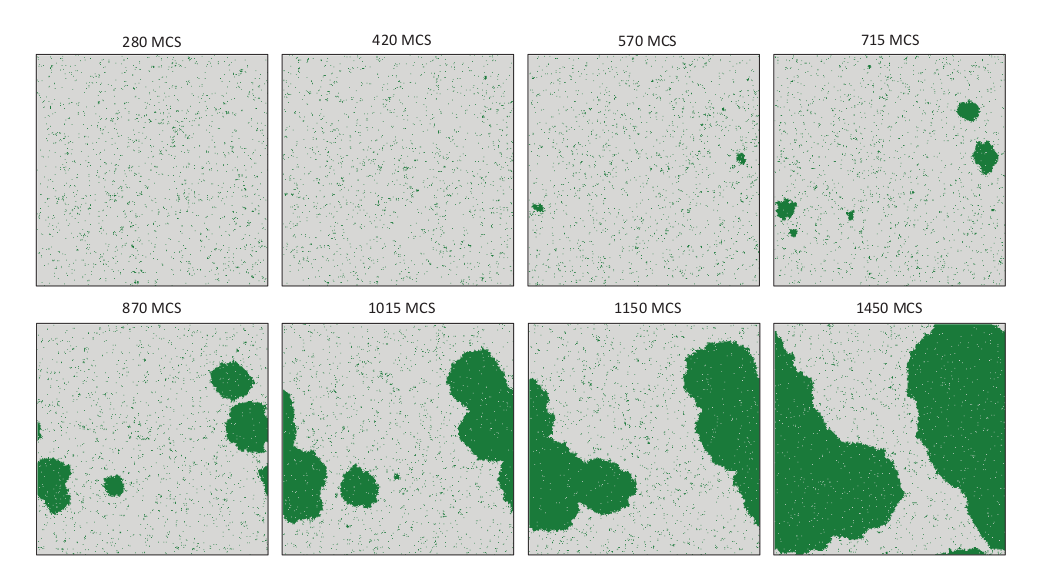
\includegraphics[height=0.4\textheight]{../resources/images/fig6.png}
		\hfill
		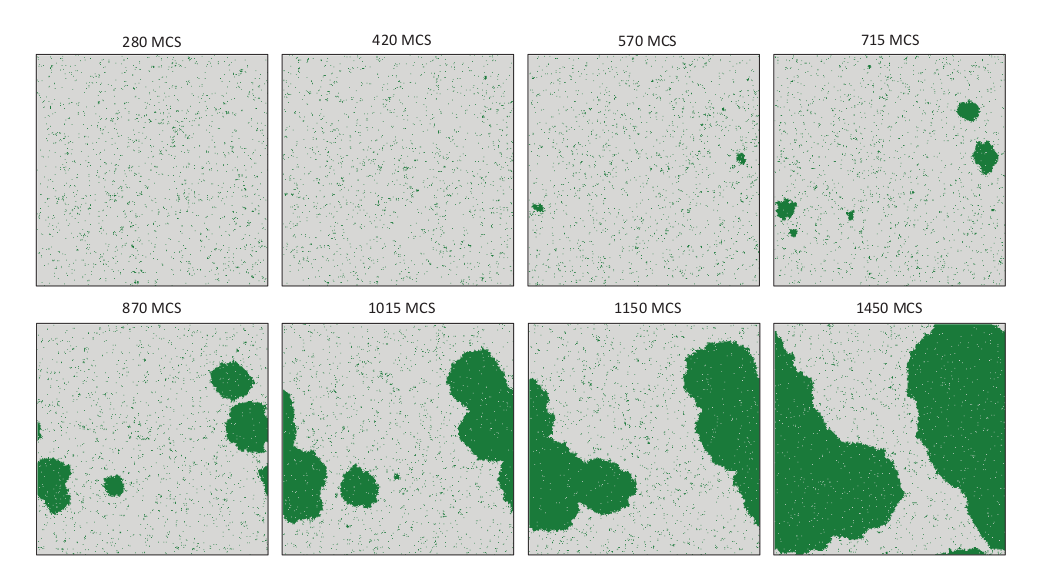
\includegraphics[height=0.4\textheight]{../resources/images/fig6.png}
		\caption{Up - publication; down - ours.}
	\end{figure}
	Comparison (Fig. 6)
	GIF!
\end{frame}

\section{Concentration in time}

\begin{frame}{Concentration}
	Concentration
	$$ c_t = \frac{N_{\uparrow}(t)}{N} $$ 
	where 
	\begin{itemize}
		\item $ N_{\uparrow}(t) $ - number of adopted people, i.e. spinsons with opinion = 1
		\item $ N $ - number of people in network
	\end{itemize}

\end{frame}

\begin{frame}{2D Lattice results}
	\begin{figure}
		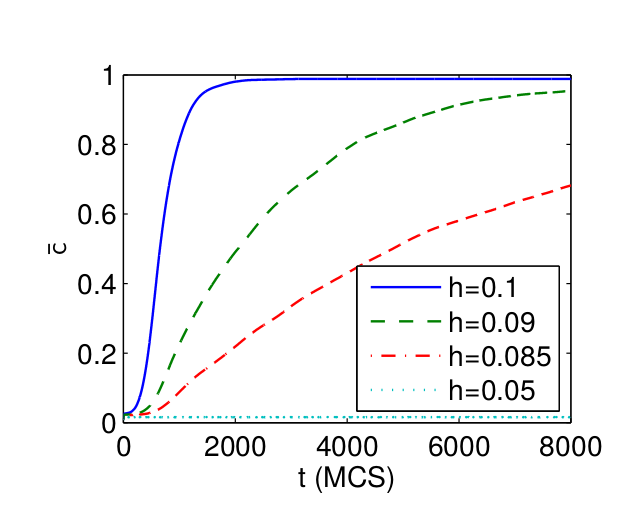
\includegraphics[width=0.475\textwidth]{../resources/images/fig7-left.png}
		\hfill
		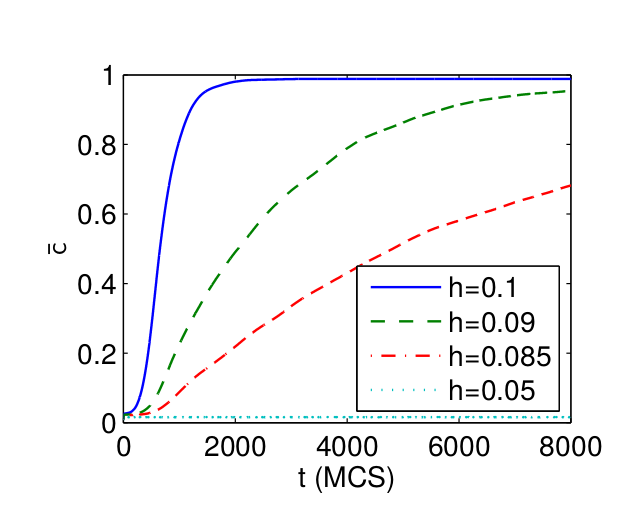
\includegraphics[width=0.475\textwidth]{../resources/images/fig7-left.png}
		\caption{Left - publication; right - ours.}
	\end{figure}
\end{frame}

\begin{frame}{Complete graph results}
	\begin{figure}
		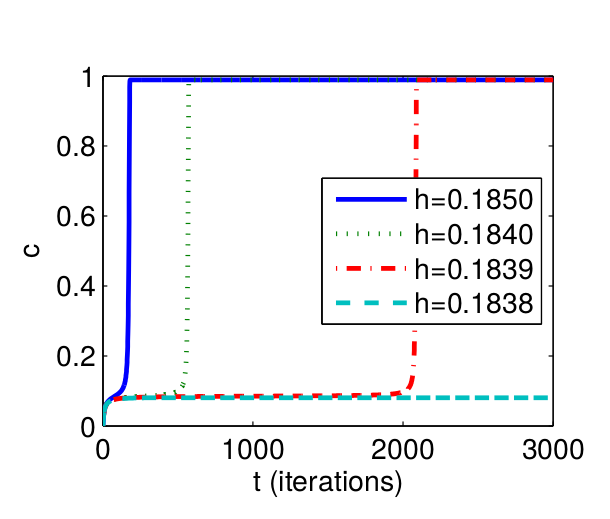
\includegraphics[width=0.475\textwidth]{../resources/images/fig10-left.png}
		\hfill
		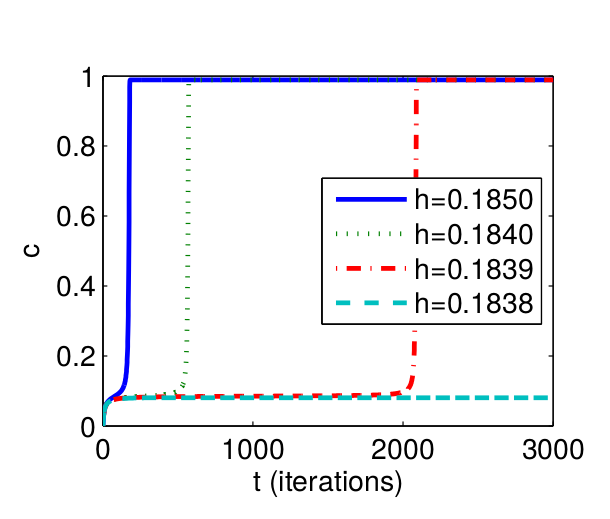
\includegraphics[width=0.475\textwidth]{../resources/images/fig10-left.png}
		\caption{Left - publication; right - ours.}
	\end{figure}
\end{frame}

\begin{frame}{Watts-Strogatz results}
	\begin{figure}
		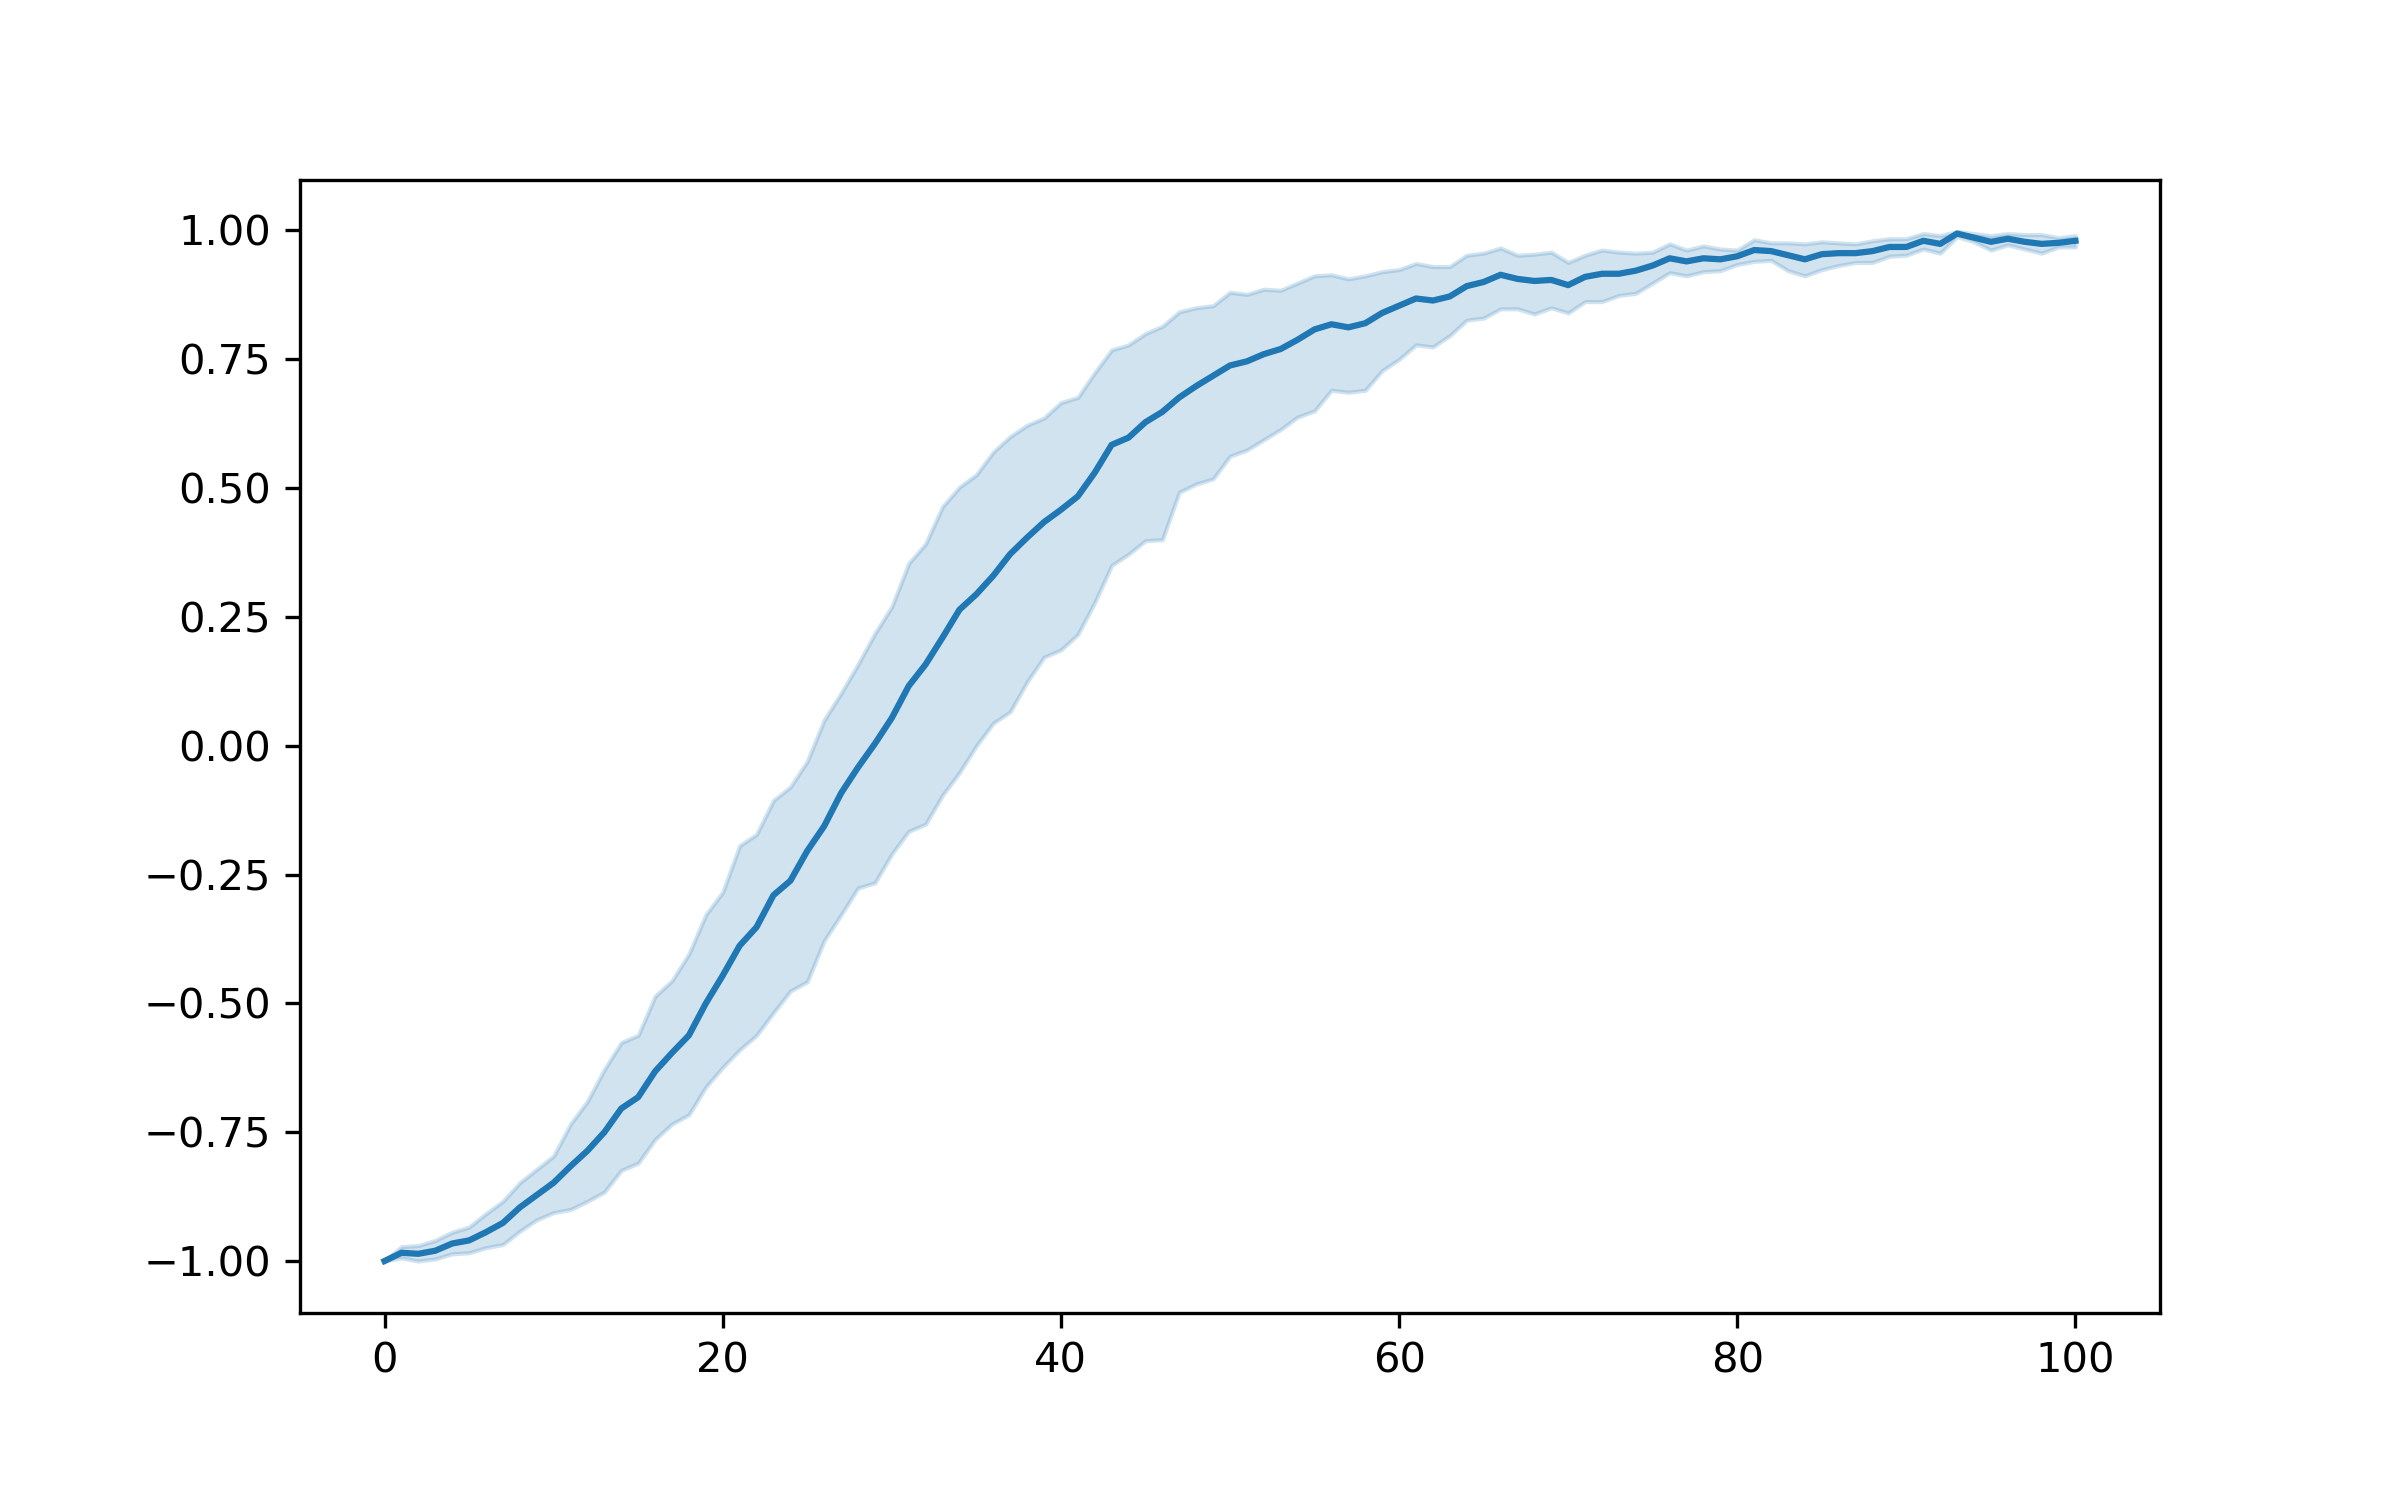
\includegraphics[width=\textwidth]{../results/images/example.png}
		\caption{Our work - simulation.}
	\end{figure}
\end{frame}

\begin{frame}{Barabasi-Albert results}
	\begin{figure}
		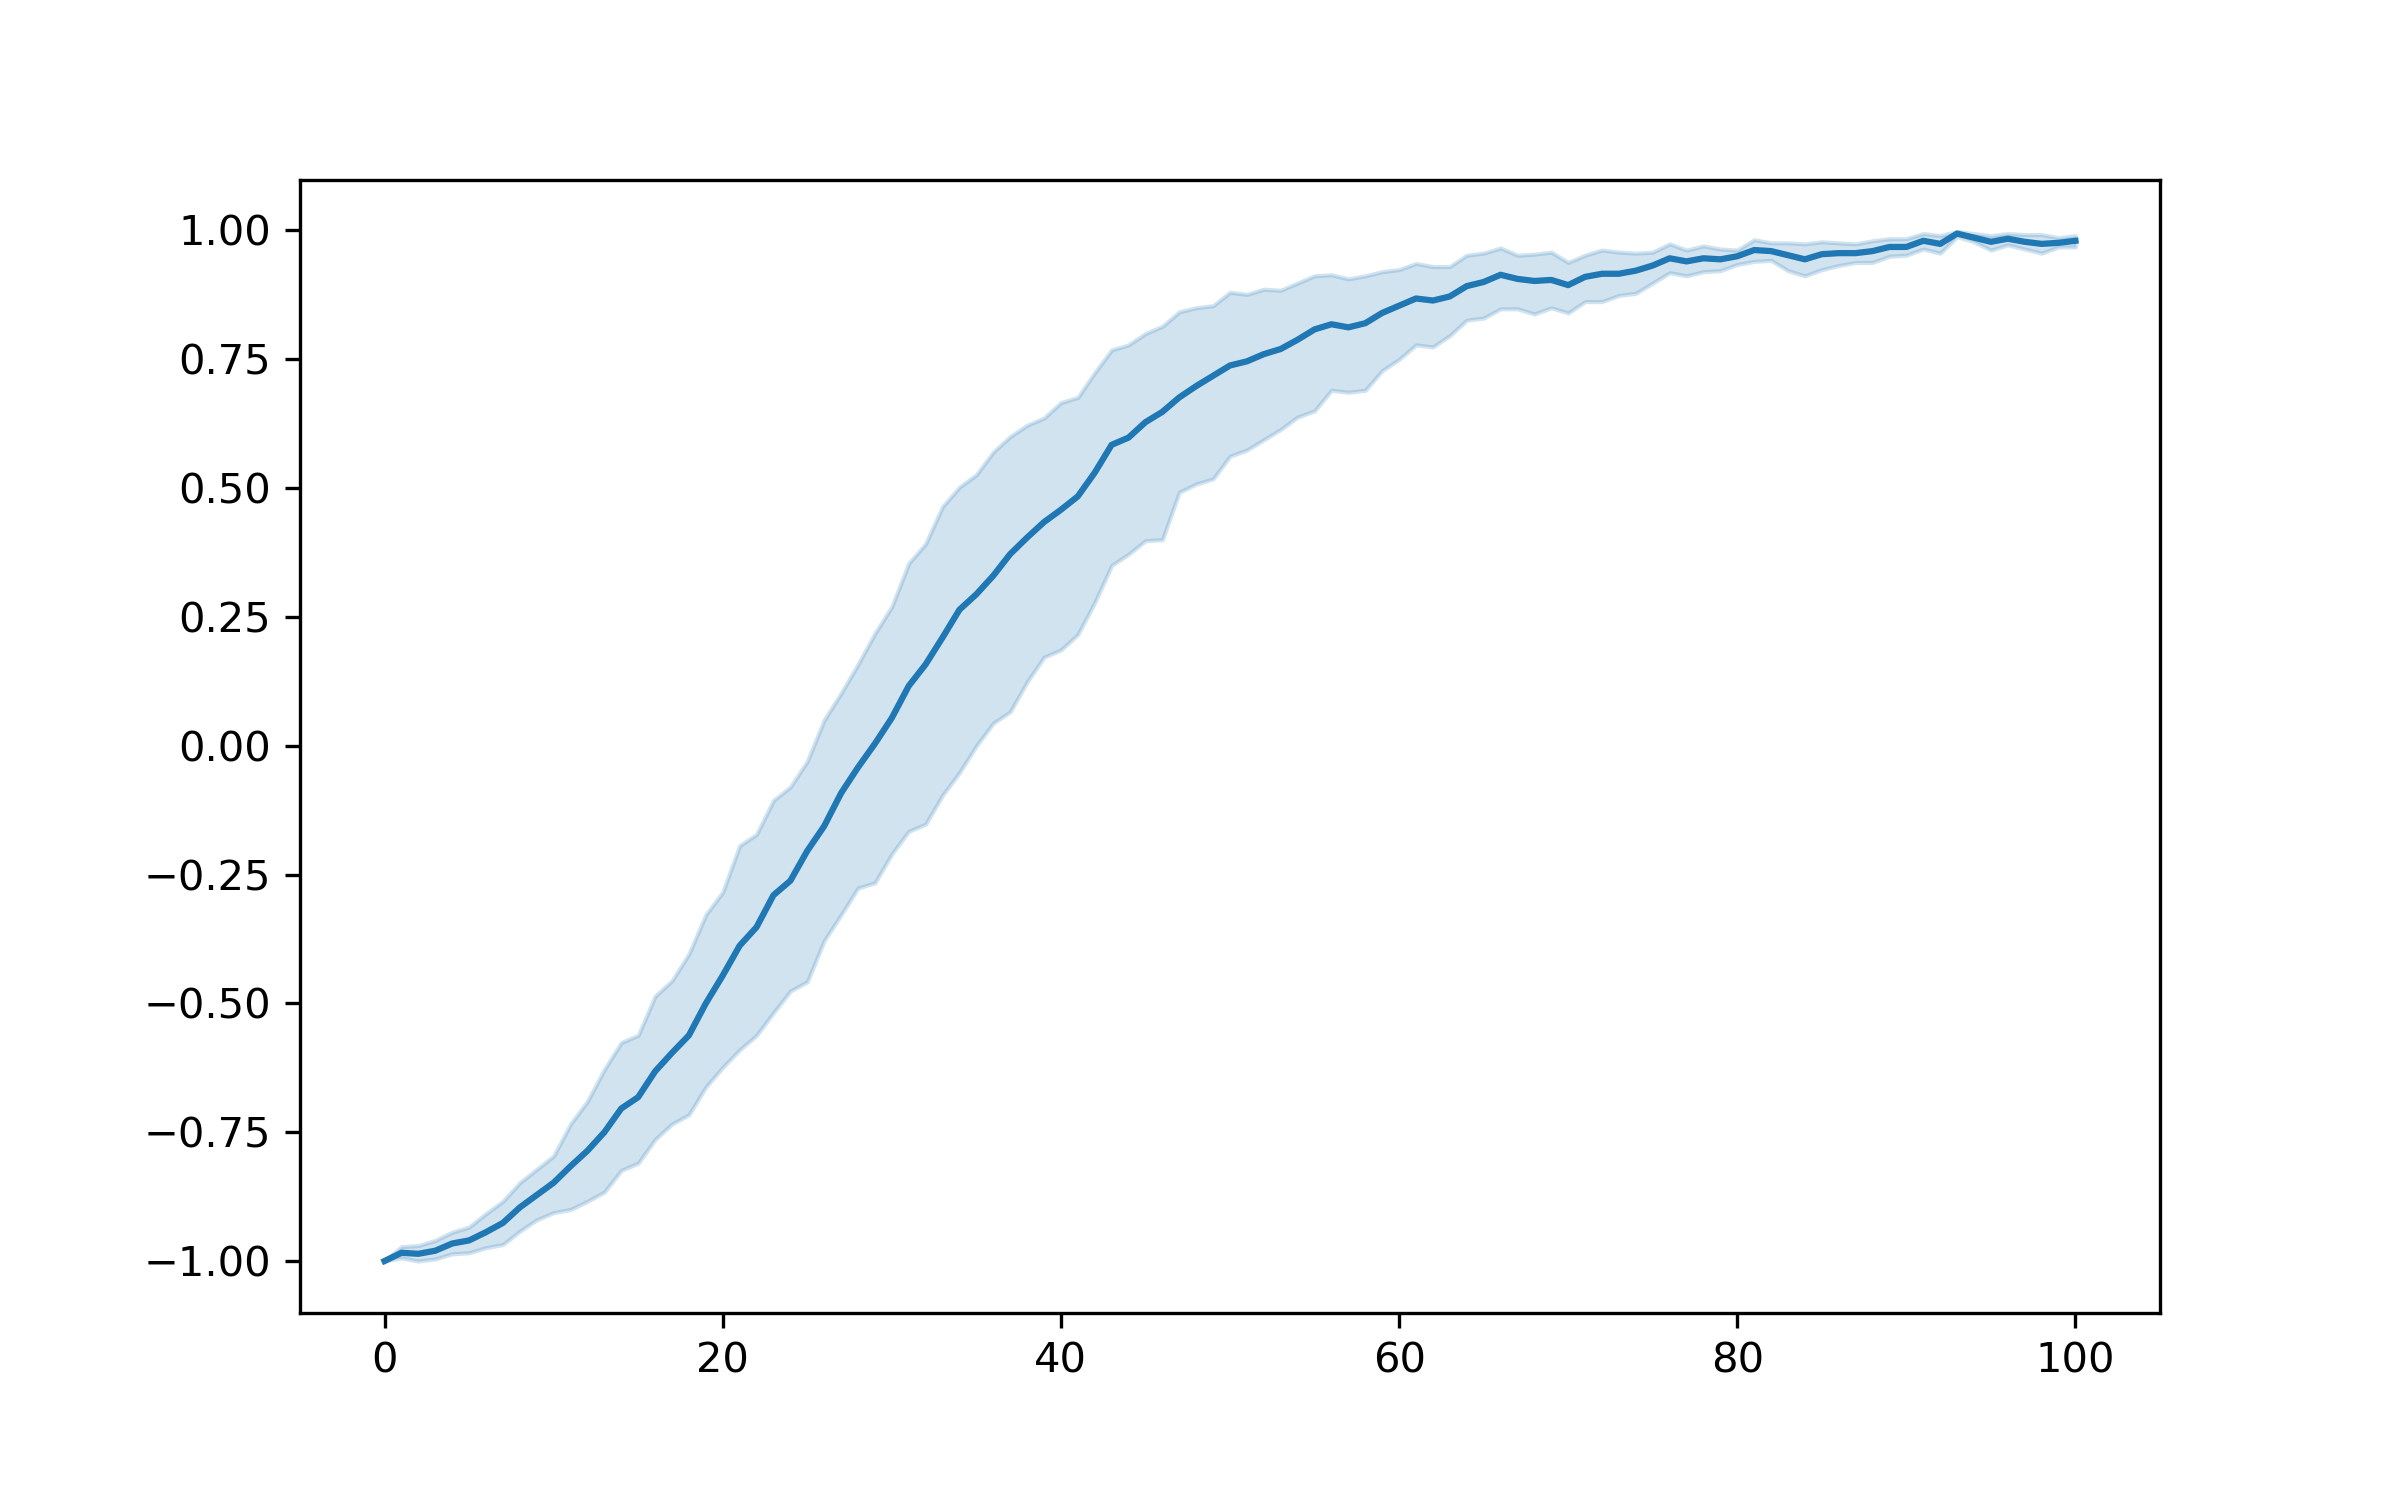
\includegraphics[width=\textwidth]{../results/images/example.png}
		\caption{Our work - simulation.}
	\end{figure}
\end{frame}

\begin{frame}{Comparison of models}
	
\end{frame}

\section{Market penetration level}

\begin{frame}{Valley of death}
	Valley of death and $h^*(p)$ description
\end{frame}

\begin{frame}{2D Lattice results}
	\begin{figure}
		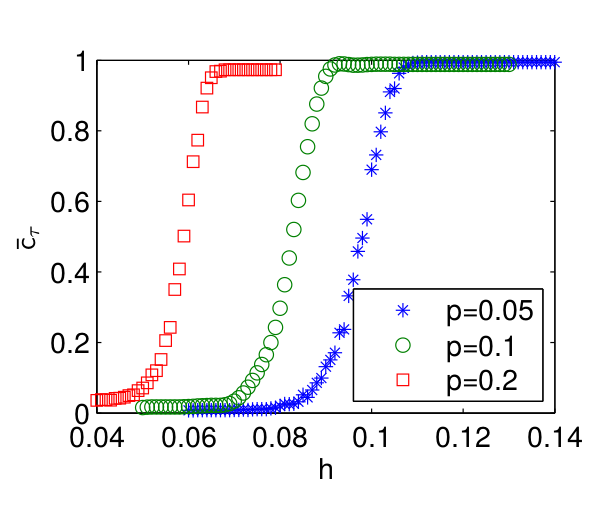
\includegraphics[width=0.475\textwidth]{../resources/images/fig9-left.png}
		\hfill
		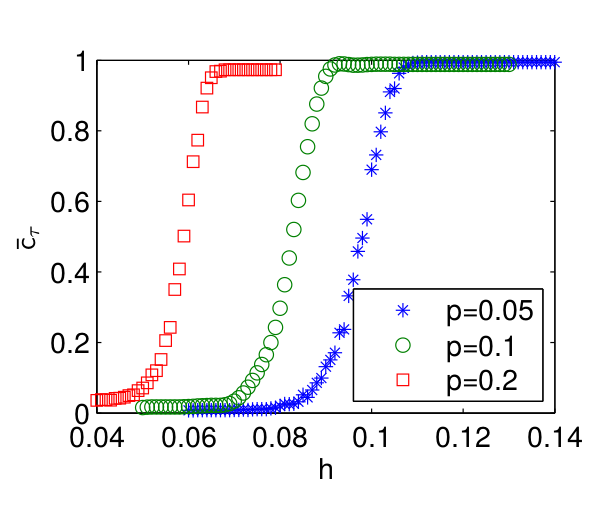
\includegraphics[width=0.475\textwidth]{../resources/images/fig9-left.png}
		\caption{Left - publication; right - ours.}
	\end{figure}
	Comparison - Fig. 9 (left)
	Simulations
\end{frame}

\begin{frame}{Complete graph results}
	\begin{figure}
		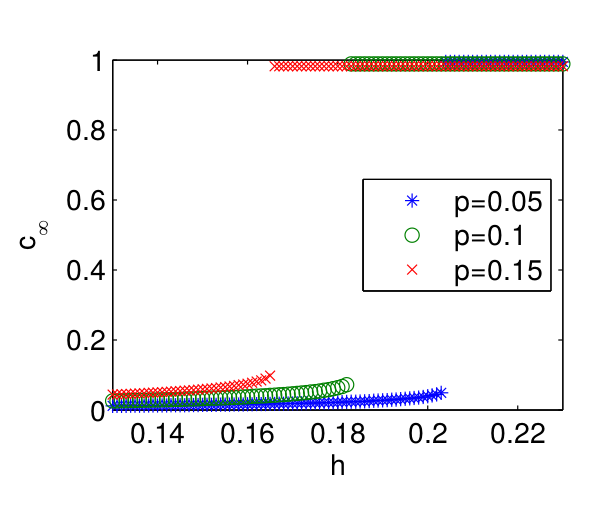
\includegraphics[width=0.475\textwidth]{../resources/images/fig10-right.png}
		\hfill
		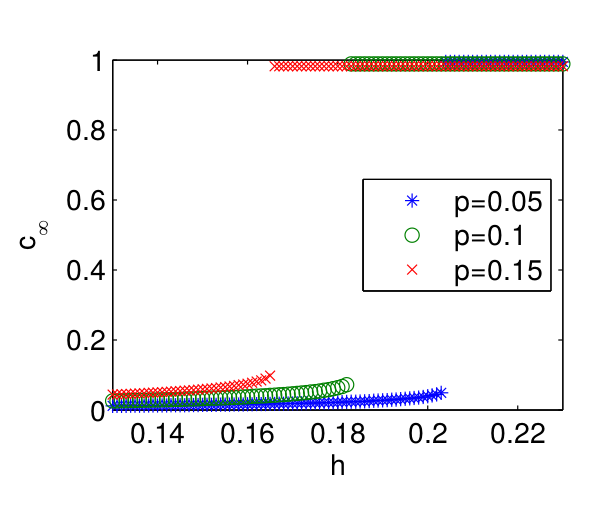
\includegraphics[width=0.475\textwidth]{../resources/images/fig10-right.png}
		\caption{Left - publication; right - ours.}
	\end{figure}
	Comparison - Fig. 10 (right)
	Theoretical results
\end{frame}

\begin{frame}{Watts-Strogatz results}
	\begin{figure}
		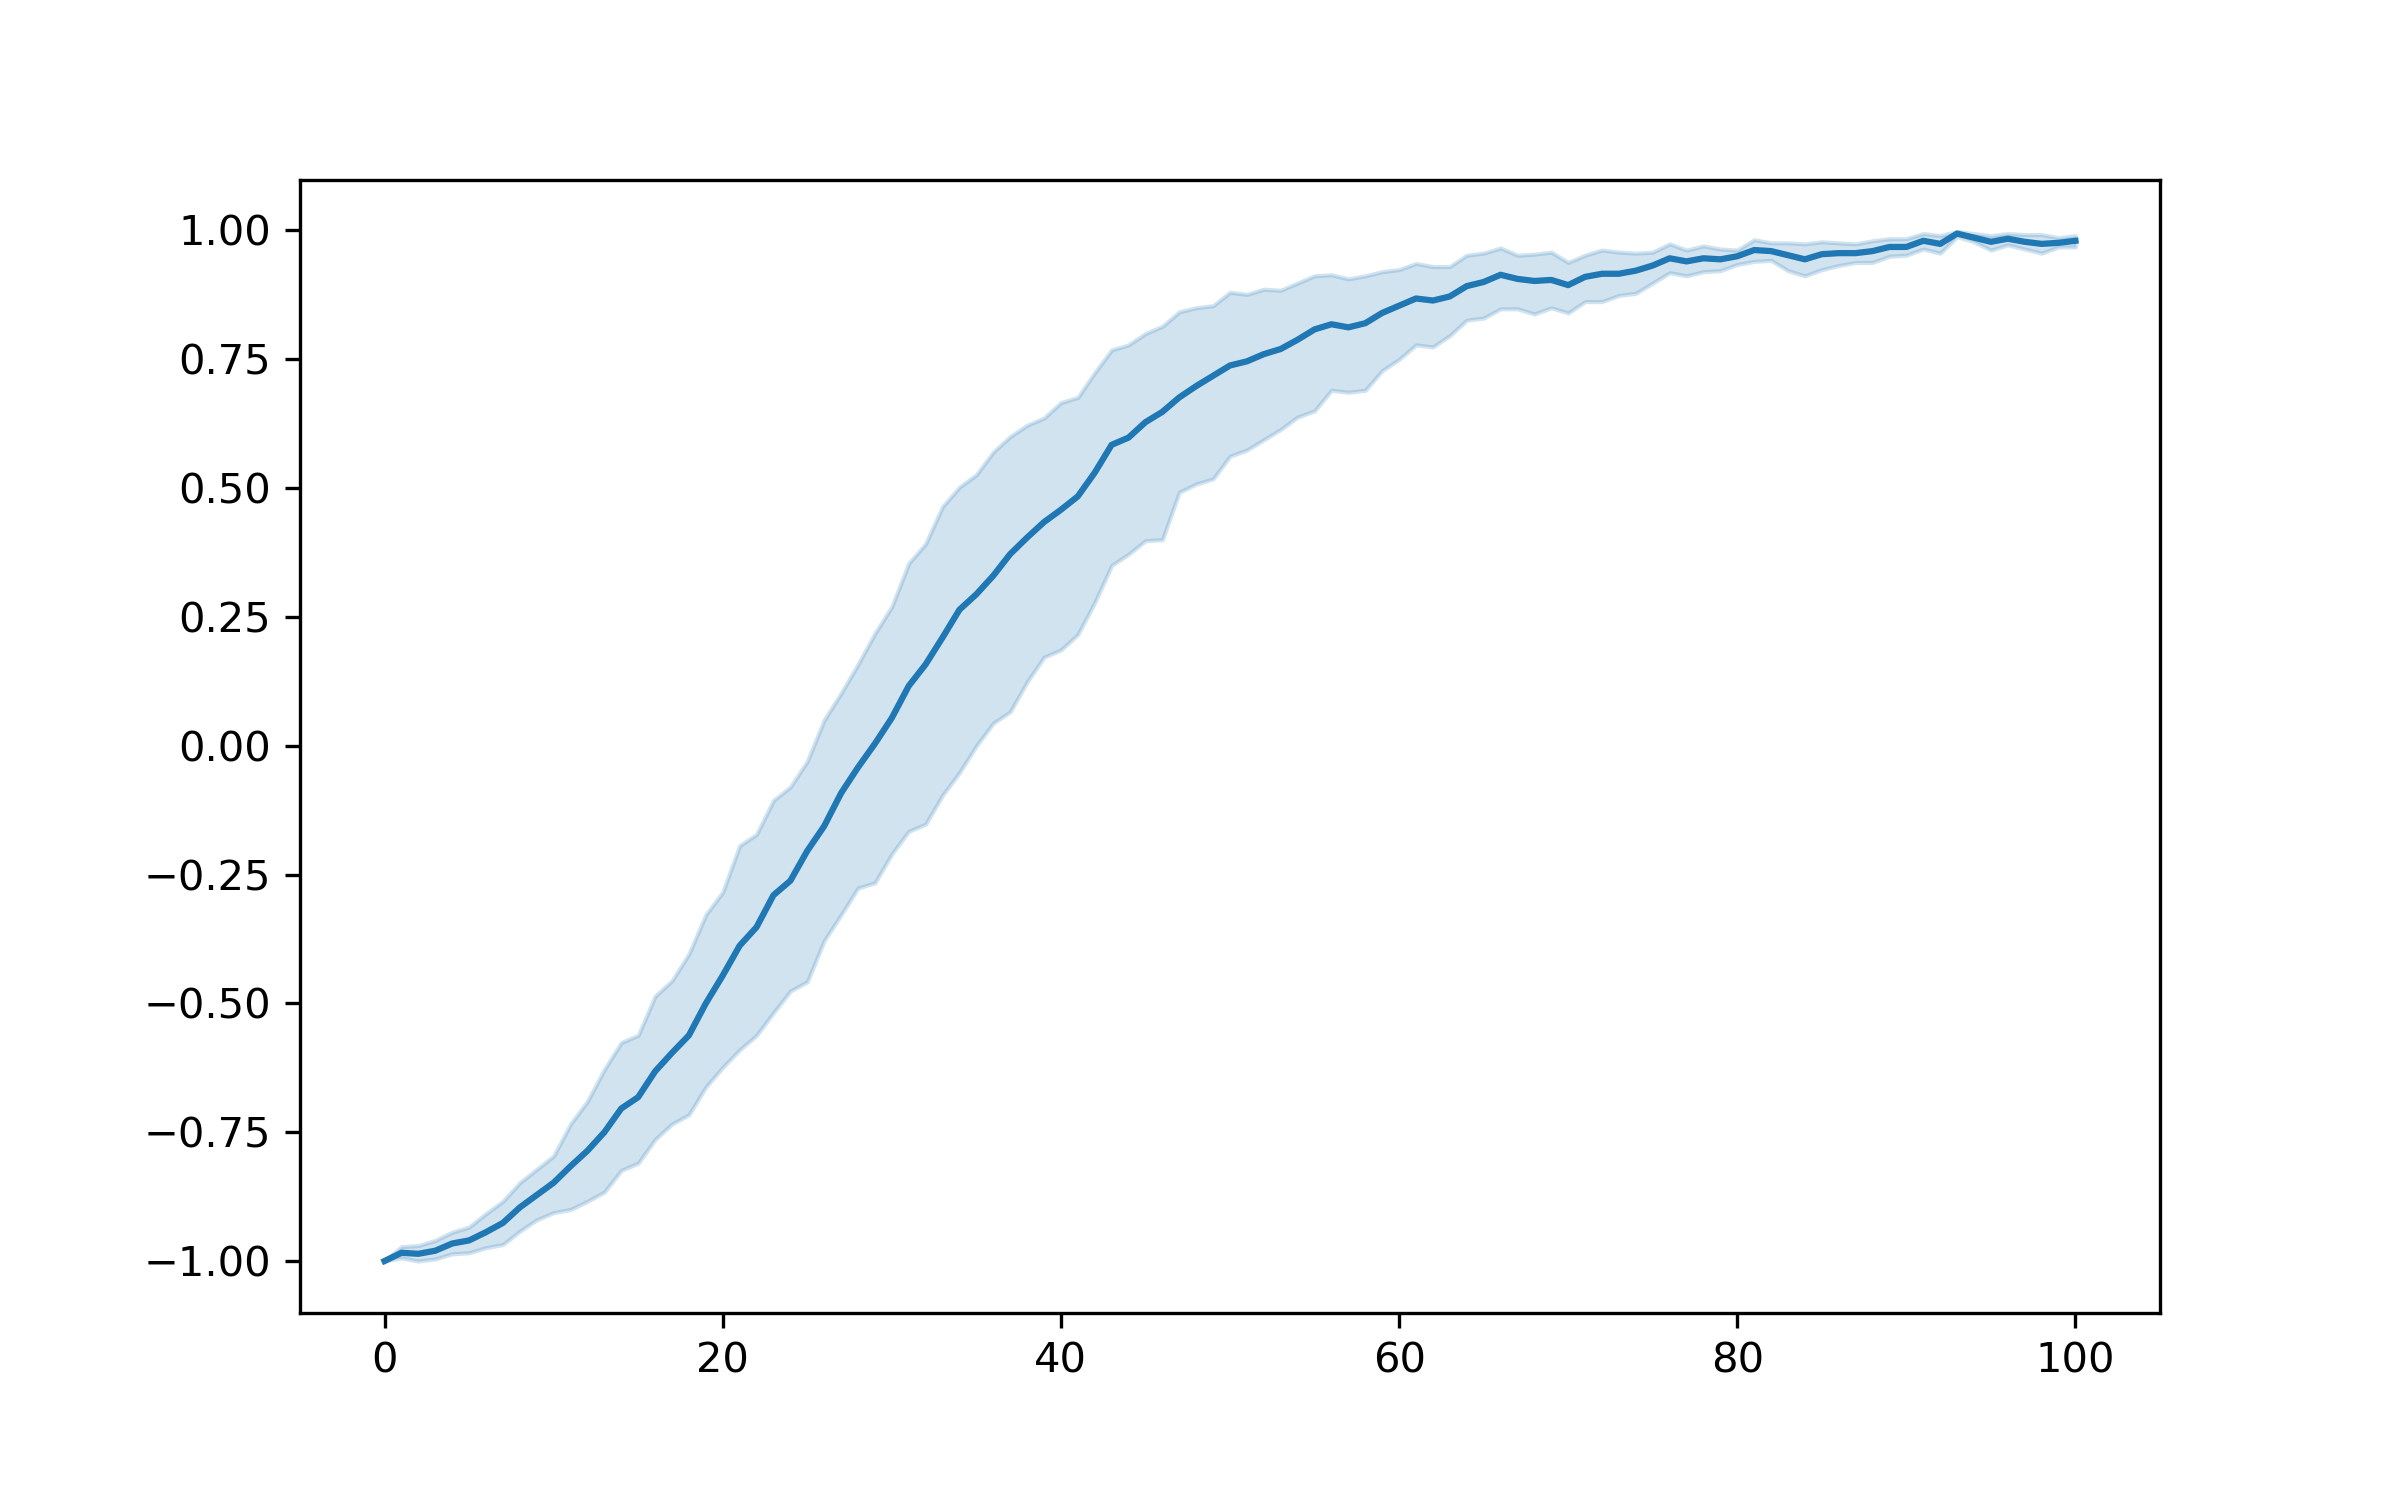
\includegraphics[width=\textwidth]{../results/images/example.png}
		\caption{Our work - simulation.}
	\end{figure}
\end{frame}

\begin{frame}{Barabasi-Albert results}
	\begin{figure}
		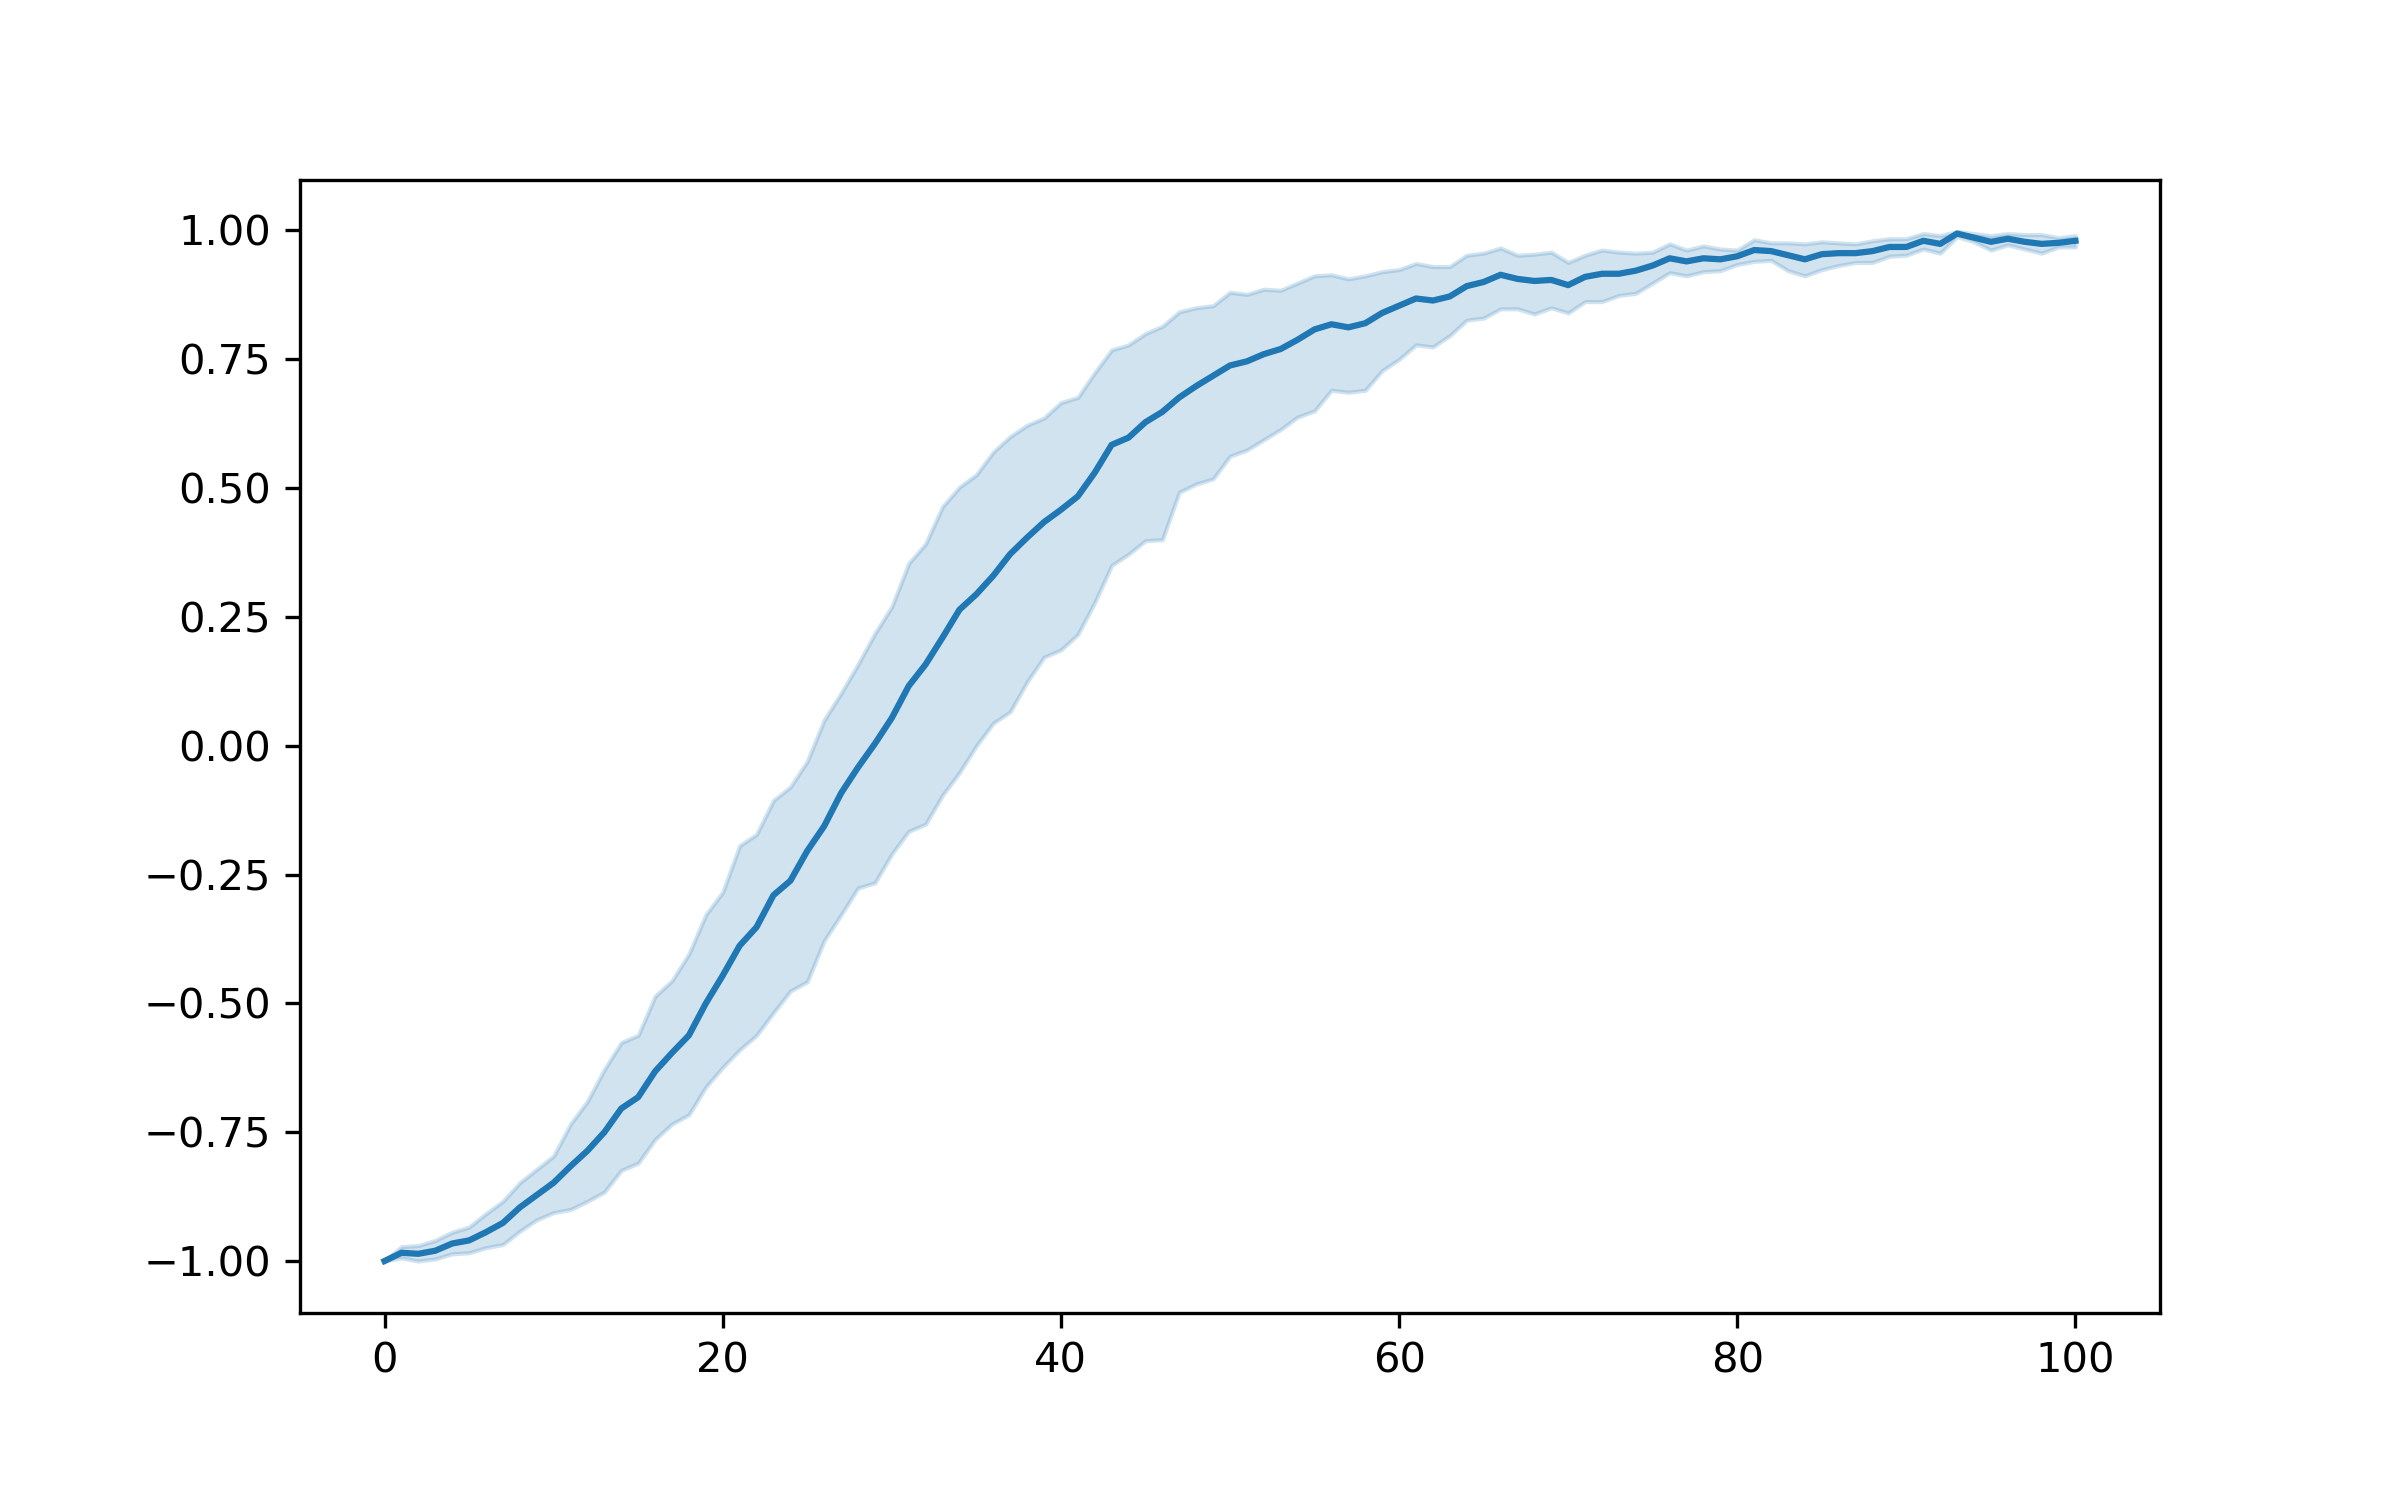
\includegraphics[width=\textwidth]{../results/images/example.png}
		\caption{Our work - simulation.}
	\end{figure}
\end{frame}

\begin{frame}{Comparison of models}
	
	Try to find universal $h$
	\begin{table}[]
		\begin{tabular}{l|llll}
			& \multicolumn{3}{c}{p} &  \\
			\hline
			Graph           & 0.05   & 0.1   & 0.2  &  \\
			\hline
			2D Lattice grid &        &       &      &  \\
			Complete graph  &        &       &      &  \\
			Watts-Strogatz  &        &       &      &  \\
			Barabasi-Albert &        &       &      & 
		\end{tabular}
	\end{table}
\end{frame}

\section{Conclusions}

\begin{frame}{Conclusions}
	content...
\end{frame}

\begin{frame}
	 \centering
	{\Large Thank you for your attention!}
	
\end{frame}

\end{document}
